\chapter{Implementation}
\label{chap:implementation}

\section{Tasks}
\label{sec:implementation.Tasks}
Die Tasks bzw. Aufgaben des Bots wurden in eigenen Klassen implementiert. Das Interface Task \footnote{das Interface ist im Code unter ants.tasks.Bot.Java auffindbar } definiert eine setup()-Methode welche den Task initiert, sowie eine perform()-Methode welche den Task ausf�hrt. Im Program werden die Tasks nach deren Wichtigkeit ausgef�hrt, was auch der nachfolgenden Reihenfolge entspricht. Jeder Task kann nur auf die unbesch�ftigten Ameisen zur Verf�gung, d.h. jene welchen noch keine Aufgabe zugeteilt wurde.

\subsection{MissionTasks}
\label{subsec:implementation.Tasks.MissionTask}
Dieser Task pr�ft alle akutellen Missionen auf deren G�ltigkeit wie zum Beispiel, ob die Ameise der Mission noch am Leben ist. Falls g�ltig, wird der n�chste Schritt der Mission ausgef�hrt.

\subsection{GatherFoodTask}
\label{subsec:implementation.Tasks.GatherFoodTask}
F�r jedes Food-Tile wird in einem definierbaren Radius r die n�chsten Ameisen bestimmt. Danach wird aufsteigend der Luftliniendistanz versucht mit dem Pfadsuchalgorithmus SiMPLE oder falls dieser kein Pfad gefunden hat mit A* eine passierbare Route gesucht. Falls diese existiert wird mit der Ameise und dem Food-Tile eine GatherFoodMission erstellt, welche die Ameise zum Food-Tile f�hrt. Zu jedem Food-Tile wir immer nur eine Ameise geschickt.

\subsection{AttackHillsTask}
\label{subsec:implementation.Tasks.AttackHillsTask}
Sobald gegnerische Ameisenhaufen sichtbar sind, sollen diese angegriffen werden, da dies +2 Punkte gibt. Die Kriterien, dass eine Pfad zum gegnerischen Haufen gesucht wird, sind die selben wie beim GatherFoodTask, ausser dass mehrere Ameisen das Ziel angreifen k�nnen. Es wird ein AttackHillMission erstellt.

\subsection{CombatTask}
\label{subsec:implementation.Tasks.CombatTask}
Beim Angriffstask wird berechnet ob wir in einem Kampfgebiet (viewRadius2) die �berhand, d.h mehr Ameisen platziert haben. Falls ja wird die gegnerische Ameise angegriffen.

\subsection{DefendAreaTask}
\label{subsec:implementation.Tasks.DefendAreaTask}
Dieser Task w�re vogesehen um eine Region wie zum Beispiel der eingene Ameisenh�gel zu sch�tzen. Dieser Task ist aber noch nicht implementiert.

\subsection{ExploreTask}
\label{subsec:implementation.Tasks.ExploreTask}
F�r alle noch unbesch�ftigten Ameisen wird mittels ManhattenDistance der n�chste Ort gesucht, der noch nicht sichtbar, also unerforscht ist. Falls ein Pfad mittels Pfadsuchalgorithmus gefunden wird, wird eine ExplorerMission/ref{sec:implementation.Missionen} erstellt, das heisst die Ameise wird den gefundenen Pfad in den n�chsten Spielz�gen ablaufen.

\subsection{FollowTask}
\label{subsec:implementation.Tasks.FollowTask}
Der FollowTask ist f�r Ameisen angedacht welche aktuell keine Aufgabe haben. Diese Ameisen sollen einfach einer besch�ftigten Ameise folgen, damit diese nicht alleine unterwegs ist.

\subsection{ClearHillTask}
\label{subsec:implementation.Tasks.ClearHillTask}
Dieser Task bewegt alle Ameisen, welche neu aus unserem H�gel "schl�pfen" und noch keinen Befehl haben, davon weg. So werden nachfolgende Ameisen nicht durch diese blockiert.

\subsection{ClusteringTask}
\label{subsec:implementation.Tasks.ClusteringTask}
Der ClusteringTask wird als Vorbereitung f�r den HPA* Algorithmus verwendet. Hier wird alle sichtbaren Kartenregionen ein Clustering vorgenommen. Das Clustering wird im Kapitel \ref{subsec:implementation.Pfadsuche.HPAstar} im Detail beschreiben.

\section{Missionen}
\label{sec:implementation.Missionen}
Eine Mission dauert �ber meherer Spielz�ge. Die meisten Missionen (GatherFoodMission,ExploreMission,AttackHillMission,AttackAntMission) sind Pfadmissionen\footnote{Die abstrakte Klasse PathMission ist im Code unter ants.missions.PathMission.java auffindbar } bei welchen die Ameise einem vorgegebenen Pfad, der bereits beim Erstellen der Mission berechnet wurde, folgt. Je nach spezifischer Mission sind aber die Abbruchbedingungen anders. Zum Beispiel die GatherFoodMission ist nur solange g�ltig wie das Futter noch nicht von einer anderen Ameise eingesammelt wurde.



\section{Pfadsuche}
\label{sec:implementation.Pfadsuche}
Wir haben drei m�gliche Pfadalgorithmen in unserem Code eingebaut. Via Klasse PathFinder kann f�r die Pfadsuche der Alogrithmus ausgew�hlt werden.


\subsection{Simple Algorthmus}
\label{subsec:implementation.Pfadsuche.Simple}

Der Simple Algorithmus versucht das Ziel zu erreichen indem er zuerst die eine, dann die andere Achse abl�uft. Sobald ein Hindernis in den Weg kommt bricht der Algorithmus ab. Im folgenden Beispiel sucht der Alogrithmus den Vertikal-Horizontal Pfad. Da dieser Pfad wegen dem Wasserhindernis (blau) nicht ans Ziel f�hrt, wird via Horizontal-Vertikal Pfad gesucht. Hier wird der Pfad gefunden. Dieser Algorithmus ist wie der Name sagt sehr einfach aufgebaut und kostet wenig Rechenzeit. Daf�r kann er keinen Hindernissen ausweichen.

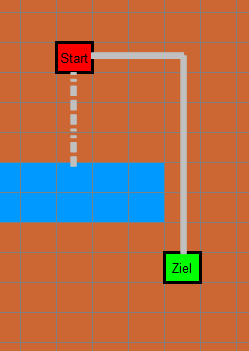
\includegraphics[height=50mm]{bilder/simplepath.png}


\subsection{A* Algorthmus}
\label{subsec:implementation.Pfadsuche.Astar}
Beim A* Algorithmus wird f�r jeden expandierten Knoten einen heuristischen Wert f(x) f�r gesamte Pfadl�nge berechnet. Dass heisst f(x) besteht aus einem Teil g(x) welches die effektiven Kosten vom Startknoten zum aktuellen Knoten berechnet. Der andere Teil ist ein heuristischer Wert der Pfadkosten welche bis zum Zielknoten noch anfallen werden. Dieser Wert muss die effektiven Kosten zum Ziel immer untersch�tzen. Dies ist in unserem Spiel dadurch gegeben, dass sich die Ameisen nicht diagonal bewegen k�nnen, wir aber f�r den heuristischen Wert die Luftlinie zum Ziel nehmen. Die Pfadsuche wird immer bei dem Knoten fortgesetzt welcher die kleinsten Kosten f(x) hat.

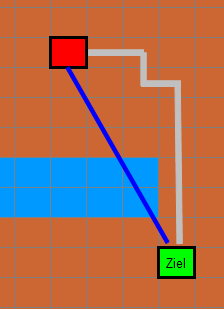
\includegraphics[height=50mm]{bilder/heuristicAstar.png}

Das Bild zeigt, dass der effektive Pfad (grau) vom expandierenden roten Knoten minimal 10 Pixel lang sein kann. Die Luftlinie (blau) als heurstischer Pfad hat aber nur die L�nge 7.6 Pixel. Damit erf�llt unsere Implementation die Anforderungen des Algorithmus.

Dieser Algorithmus wird in unserem Code f�r eine Pfadsuche �ber alle Pixel (jedes Pixel ist ein Node) verwendet aber auch f�r die berechneten Kanten welche im HPA* verwendet werden.

\subsection{HPA* Algorthmus}
\label{subsec:implementation.Pfadsuche.HPAstar}

Eine Pfadsuche A* �beralle Pixel ist sehr teuer, da es viel Pfade gibt, die zum Teil nur ein Pixel nebeneinander liegen. Es werden bis zum Schluss verschiedenen Pfaden nachgegangen. Abhilde zu dieser sehr feinmaschigen Pfadsuche bietet der HPA* bei welchem im sogenanten Clustering �bermehrere Pixel verlaufende Kanten und Knoten berechnet werden.

\title{Clustering}


\section{JavaScript Addon f�r HMTL-Gameviewer}
\label{sec:implementation.Addon}
TODO
